\documentclass[a4paper,11pt,titlepage]{jsarticle}

% 画像
\usepackage[dvipdfmx]{graphicx}
\usepackage{here}

\begin{document}
205721C Haruki Oshiro

\section{2-3 results}
Figure 1 is a graph of fileread results.
\begin{itemize}
    \item "1st read" is the speed of the first 
        file read.
    \item "2nd read" is the speed of the second
         file read.
\end{itemize}
 
From Figure1, it can be seen that "2nd read"
 time is faster than "1st read" time.

The cache is used when reading the file for the second time.
So it is considered that "2nd read" became faster than "1st read"
due to the cache.

\begin{figure}[H]
    \centering
    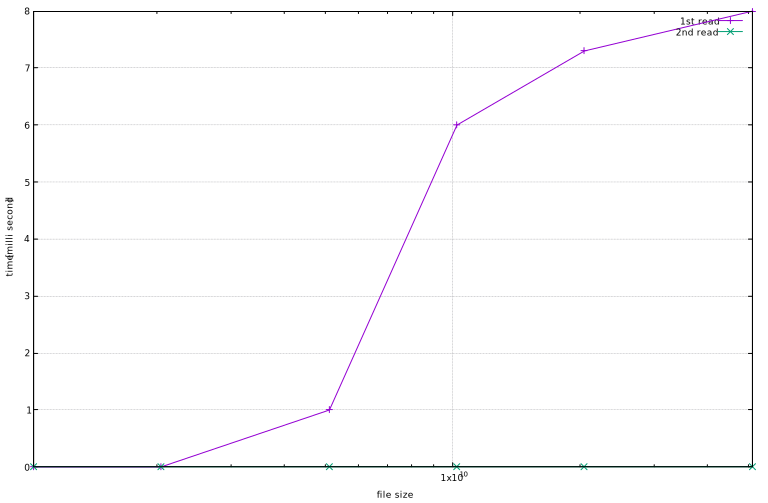
\includegraphics[scale=0.5]{./results/os23/2-3result.pdf}
    \renewcommand{\figurename}{Figure }
    \caption{2-3 result of file read}
\end{figure}
% --- ---
\end{document}